\chapter{Problema e Proposta}


\section{Problema}
	O problema que nos propomos a resolver se refere ao fato do \textit{middleware} \textit{UbiquitOS} não ter como descobrir de forma não intrusiva se existe algum usuário presente, quem é esse usuário e onde o mesmo está dentro do \textit{SmartSpace}.

	Essas informações são importantes para o \textit{middleware} pois para conseguir uma boa interação entre as diversas peças que compõem o \textit{SmartSpace} é necessário que se tenha a disposição informações de contexto. Informações de contexto são importantes para definir ajustes finos nos componentes do ambiente como por exemplo definir o perfil e a localização do usuário e apartir daí ajustar os dispositivos presentes no ambiente.

\section{Proposta}

	Nosso objetivo é propor um sistema eficiente para reconhecimento e localização de usuários dentro de um \textit{SmartSpace} em tempo real. Para alcançar esse objetivo iremos implementar um sistema eficiente que através de imagens de cor e de profunidade providas pelo \textit{Kinect} e utilizando as bibliotecas, \textit{OpenCV} e \textit{OpenNI}, reconheça os usuários e rastrei-o durante a sua permanência no \textit{SmartSpace}.


	Ao todo usaremos 4 \textit{Kinects} dispostos conforme a Figura \ref{smartSpaceProposto}. Essa disposição foi definida para evitar problemas de obstrução de usuários que podem atrapalhar o reconhecimento e o rastreamento dos usuários e também para maximizar o alcance dos \textit{Kinects} e almentar a robustez graças a redundância de dados.

	\begin{figure}[hbt]
		\begin{center}
			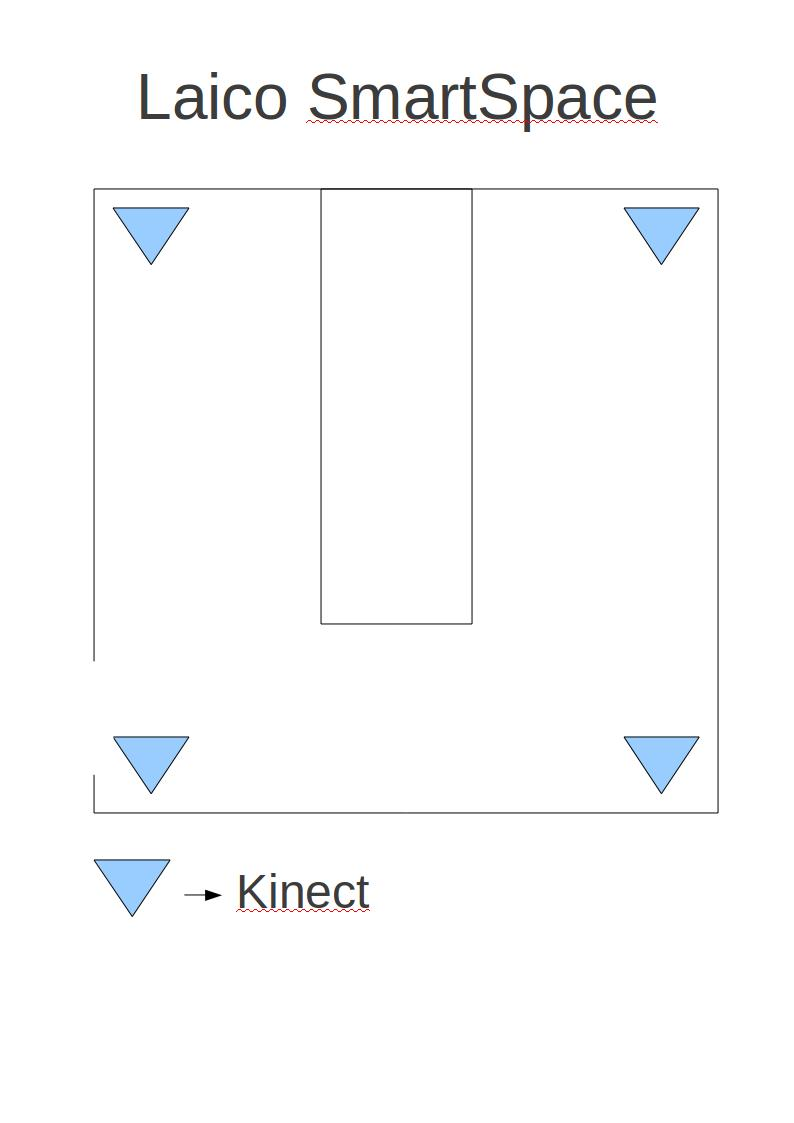
\includegraphics[scale=0.3]{figuras/4.ProblemaEProposta/esquemaSmartSpaceProposto.jpg}
		\end{center}
		\caption{Esquema proposto para o \textit{SmartSpace} com \textit{Kinect}.}
		\label{smartSpaceProposto}
	\end{figure}

	Na nossa proposta contamos que o \textit{Eigenfaces}, método de reconhecimento facial que o \textit{OpenCV} implementa, seja suficientemente confiável e que o rastreamento fornecido pelo \textit{OpenNI} seja suficientemente robusto para a dinâmicidade do ambiente.

	A partir dessa proposta esperamos que o nosso sistema funcione em tempo real e que tenha o índice mínimo de confiança de 95\%. 